\section{Descrizione dei singoli componenti}
\subsection{Premi}
\begin{figure}[h]
\begin{center}
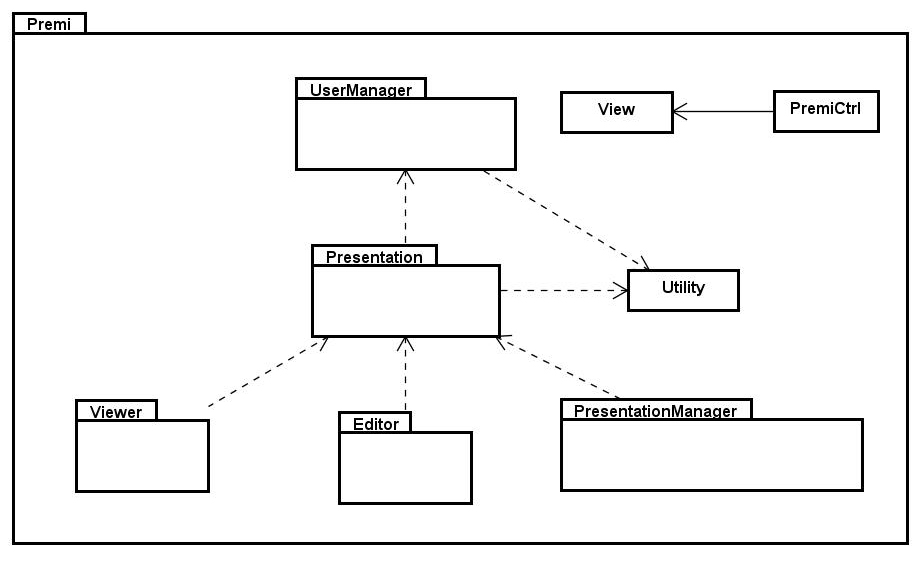
\includegraphics[scale=0.45]{img/diapkg/premi-class.jpg}
\caption{Diagramma del package Premi}
\end{center}
\end{figure}


\subsubsection{Premi.Utility}
\begin{itemize}
  \item[] \textbf{Nome:} Utility
  \item[] \textbf{Tipo:} class
  \item[] \textbf{Package:} Premi
  \item[] \textbf{Descrizione:} classe statica di utilità che fornisce strumenti per interagire con la base di dati
\end{itemize}

\subsubsection{Premi.View}
\begin{itemize}
  \item \textbf{Nome:} View
  \item \textbf{Tipo:} class
  \item \textbf{Package:} Premi
  \item \textbf{Descrizione:} view generale che funge da sfondo per le altre view
\end{itemize}

\subsubsection{Premi.PremiCtrl}
\begin{itemize}
  \item \textbf{Nome:} PremiCtrl
  \item \textbf{Tipo:} class
  \item \textbf{Package:} Premi
  \item \textbf{Descrizione:} controller generale che modifica la view principale in base alle scelte dell'utente
  \item \textbf{Relazioni con altri componenti:} la classe altera l'aspetto di \code{Premi.View} caricando le view di cui l'utente ha bisogno 
\end{itemize}

\subsection{Premi.UserManager}
\begin{figure}[h]
\begin{center}
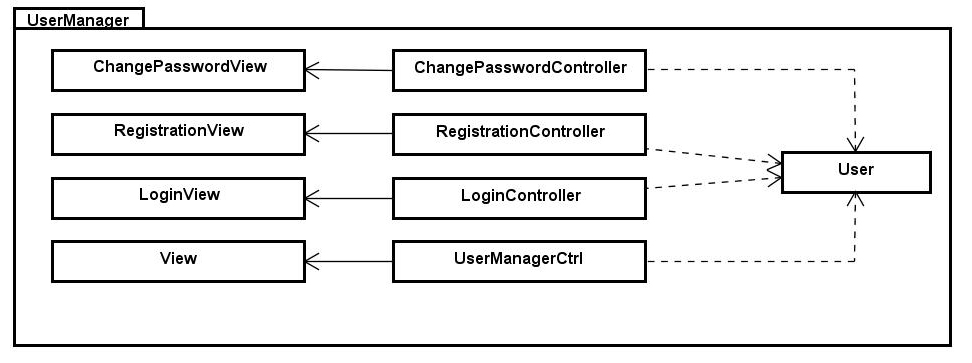
\includegraphics[scale=0.45]{img/diapkg/usermanager-class.jpg}
\caption{Diagramma del package Premi.UserManager}
\end{center}
\end{figure}
\clearpage
\subsubsection{Premi.UserManager.User}
\begin{figure}[h]
\begin{center}
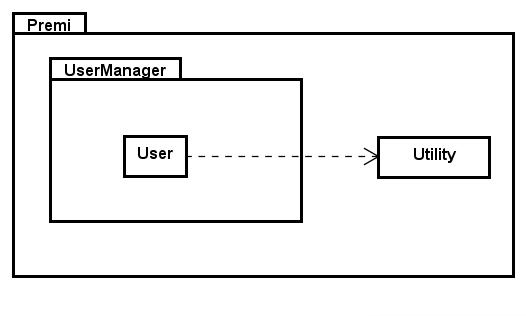
\includegraphics[scale=0.45]{img/diapkg/Utility_UserManager.jpg}
\caption{Diagramma delle dipendenze della classe User.}
\end{center}
\end{figure}
\begin{itemize}
  \item \textbf{Nome:} User
  \item \textbf{Tipo:} class
  \item \textbf{Package:} Premi.UserManger
  \item \textbf{Descrizione:} classe che definisce un utente e fornisce le funzionalità necessarie alla sua creazione, al suo login e ad un eventuale cambio di password
  \item \textbf{Relazioni con altri componenti:} si collega a \code{Premi.Utility} per le interazioni con la base di dati
\end{itemize}

\subsubsection{Premi.UserManager.View}
\begin{itemize}
  \item \textbf{Nome:} View
  \item \textbf{Tipo:} class
  \item \textbf{Package:} Premi.UserManger
  \item \textbf{Descrizione:} vista generale del package$_G$ \code{UserManager}. Puo' contenere le view abbinate alle funzionalità di \code{User}
\end{itemize}
\subsubsection{Premi.UserManager.UserManagerCtrl}
\begin{itemize}
  \item \textbf{Nome:} UserManagerCtrl
  \item \textbf{Tipo:} class
  \item \textbf{Package:} Premi.UserManager
  \item \textbf{Descrizione:} controller generale del package$_G$ \code{UserManager} dedicato a fornire alla view strumenti per l'interazione con l'utente
  \item \textbf{Relazioni con altri componenti:} si collega a \code{Premi.UserManager.View} per mostrare i dati dell'utente che va a prelevare tramite {Premi.UserManager.User}
\end{itemize}
\subsubsection{Premi.UserManager.LoginView}
\begin{itemize}
  \item \textbf{Nome:} LoginView
  \item \textbf{Tipo:} class
  \item \textbf{Package:} Premi.UserManager
  \item \textbf{Descrizione:} view che permette all'utente di effettuare la login
\end{itemize}
\subsubsection{Premi.UserManager.LoginController}
\begin{itemize}
  \item \textbf{Nome:} LoginController
  \item \textbf{Tipo:} class
  \item \textbf{Package:} Premi.UserManager
  \item \textbf{Descrizione:} fornisce gli strumenti necessari alla view per effettuare la login
  \item \textbf{Relazioni con altri componenti:} è il controller dedicato di \code{Premi.UserManager.LoginView} e utilizza \code{Premi.UserManager.User} per trasmettere e ricevere le informazioni relative al login
\end{itemize}
\subsubsection{Premi.UserManager.RegistrationView}
\begin{itemize}
  \item \textbf{Nome:} RegistrationView
  \item \textbf{Tipo:} class
  \item \textbf{Package:} Premi.UserManager
  \item \textbf{Descrizione:} view che permette all'utente di registrarsi nel sistema
\end{itemize}
\subsubsection{Premi.UserManager.RegistrationController}
\begin{itemize}
  \item \textbf{Nome:} RegistrationController
  \item \textbf{Tipo:} class
  \item \textbf{Package:} Premi.UserManager
  \item \textbf{Descrizione:} fornisce gli strumenti necessari alla view per registrare l'utente
  \item \textbf{Relazioni con altri componenti:} è il controller dedicato di \code{Premi.UserManager.RegistrationView} e utilizza \code{Premi.UserManager.User} per trasmettere le informazioni relative alla registrazione
\end{itemize}
\subsubsection{Premi.UserManager.ChangePasswordView}
\begin{itemize}
  \item \textbf{Nome:} ChangePasswordView
  \item \textbf{Tipo:} class
  \item \textbf{Package:} Premi.UserManager
  \item \textbf{Descrizione:} view che permette all'utente di cambiare la propria password
\end{itemize}
\subsubsection{Premi.UserManager.ChangePasswordController}
\begin{itemize}
  \item \textbf{Nome:} ChangePassword
  \item \textbf{Tipo:} class
  \item \textbf{Package:} Premi.UserManager
  \item \textbf{Descrizione:} fornisce gli strumenti necessari alla view per cambiare la password dell'utente
  \item \textbf{Relazioni con altri componenti:} è il controller dedicato di \code{Premi.UserManager.ChangePasswordView} e utilizza  \code{Premi.UserManager.User} per trasmettere le informazioni relative al cambio password
\end{itemize}



\clearpage
\subsection{Premi.Viewer}
\begin{figure}[h]
\begin{center}
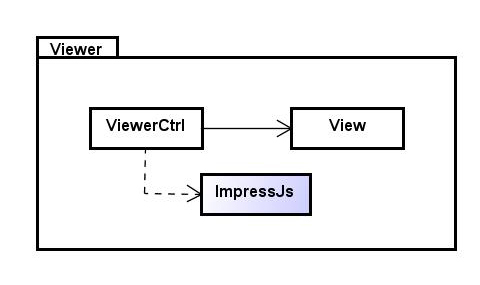
\includegraphics[scale=0.45]{img/diapkg/viewer-class.jpg}
\caption{Diagramma del package Premi.Viewer}
\end{center}
\end{figure}

\subsubsection{Premi.Viewer.View}
\begin{itemize}
  \item \textbf{Nome:} View
  \item \textbf{Tipo:} class
  \item \textbf{Package:} Premi.Viewer
  \item \textbf{Descrizione:} view che mostra la presentazione all'utente, offrendo funzionalità dipendenti dalla visibilità(pubblica o privata) o dal contesto in cui si trova(presentazione live) 
\end{itemize}
\subsubsection{Premi.ViewerCtrl}
\begin{itemize}
  \item \textbf{Nome:} ViewerCtrl
  \item \textbf{Tipo:} class
  \item \textbf{Package:} Premi.Viewer
  \item \textbf{Descrizione:} abilita funzionalità nella view in base all'utente
  \item \textbf{Relazioni con altri componenti:} è il controller dedicato di \code{Premi.Viewer.View}, utilizza  \code{Premi.UserManager.User} per verificare se l'utente è il proprietario della presentazione, e la libreria$_G$ esterna \code{ImpressJs} per aggiungere animazioni alla presentazione
\end{itemize}




\clearpage
\subsection{Premi.Presentation}
\begin{figure}[h]
\begin{center}
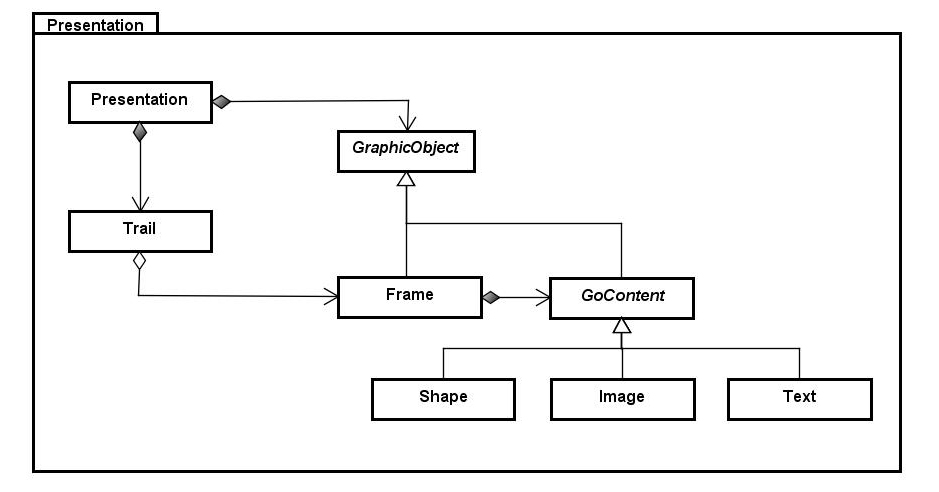
\includegraphics[scale=0.45]{img/diapkg/presentation-class.jpg}
\caption{Diagramma del package Premi.Presentation}
\end{center}
\end{figure}
\subsubsection{Premi.Presentation.GraphicObject}
\begin{itemize}
  \item \textbf{Nome:} GraphicObject
  \item \textbf{Tipo:} \textit{abstract class}
  \item \textbf{Package:} Premi.Presentation
  \item \textbf{Descrizione:} rappresenta gli oggetti grafici nella presentazione
\end{itemize}
\subsubsection{Premi.Presentation.GoContent}
\begin{itemize}
  \item \textbf{Nome:} GoContent
  \item \textbf{Tipo:} \textit{abstract class}
  \item \textbf{Package:} Premi.Presentation
  \item \textbf{Descrizione:} rappresenta gli oggetti grafici con contenuto di una presentazione
  \item \textbf{Relazioni con altri componenti:} estende \code{Premi.Presentation.GraphicObject}
\end{itemize}
\subsubsection{Premi.Presentation.Text}
\begin{itemize}
  \item \textbf{Nome:} Text
  \item \textbf{Tipo:} class
  \item \textbf{Package:} Premi.Presentation
  \item \textbf{Descrizione:} rappresenta un'area di testo nella presentazione
    \item \textbf{Relazioni con altri componenti:} estende \code{Premi.Presentation.GoContent}
\end{itemize}
\subsubsection{Premi.Presentation.Image}
\begin{itemize}
  \item \textbf{Nome:} Image
  \item \textbf{Tipo:} class
  \item \textbf{Package:} Premi.Presentation
  \item \textbf{Descrizione:} rappresenta un'immagine nella presentazione
      \item \textbf{Relazioni con altri componenti:} estende \code{Premi.Presentation.GoContent}
\end{itemize}
\subsubsection{Premi.Presentation.Shape}
\begin{itemize}
  \item \textbf{Nome:} Shape
  \item \textbf{Tipo:} class
  \item \textbf{Package:} Premi.Presentation
  \item \textbf{Descrizione:} rappresenta una figura nella presentazione. Uno shape può avere forme diverse come un quadrato, un cerchio, una freccia. Può diventare un elemento di abbellimento o di aumento dell' informazione che si vuole rappresentare. 
      \item \textbf{Relazioni con altri componenti:} estende \code{Premi.Presentation.GoContent}
\end{itemize}
\subsubsection{Premi.Presentation.Frame}
\begin{itemize}
  \item \textbf{Nome:} Frame
  \item \textbf{Tipo:} class
  \item \textbf{Package:} Premi.Presentation
  \item \textbf{Descrizione:} rappresenta un frame$_G$ nella presentazione
  \item \textbf{Relazioni con altri componenti:} estende \code{Premi.Presentation.GraphicObject} e possiede un insieme di oggetti \code{Premi.Presentation.GoContent}
\end{itemize}
\subsubsection{Premi.Presentation.Trail}
\begin{itemize}
  \item \textbf{Nome:} Trail
  \item \textbf{Tipo:} class
  \item \textbf{Package:} Premi.Presentation
  \item \textbf{Descrizione:} rappresenta un percorso nella presentazione
  \item \textbf{Relazioni con altri componenti:} possiede una lista di riferimenti ad oggetti di tipo \code{Premi.Presentation.Frame}, ma non è in possesso degli oggetti stessi
\end{itemize}
\subsubsection{Premi.Presentation.Presentation}
\begin{itemize}
  \item \textbf{Nome:} Presentation
  \item \textbf{Tipo:} class
  \item \textbf{Package:} Premi.Presentation
  \item \textbf{Descrizione:} rappresenta una presentazione
  \item \textbf{Relazioni con altri componenti:} possiede una lista di oggetti \code{premi.Presentation.GraphicObject} che possono essere sia Frame$_G$ che oggetti grafici generici e assieme compongono l'infografica$_G$ della presentazione, possiede inoltre una lista di percorsi e quindi di oggetti \code{Premi.Presentation.Trail}, identifica l'appartenenza di una presentazione ad un determinato \code{Premi.UserManager.User} e si collega alla base di dati tramite la classe statica \code{Premi.Utility}
\end{itemize}


\clearpage
\subsection{Premi.PresentationManager}
\begin{figure}[h!]
\begin{center}
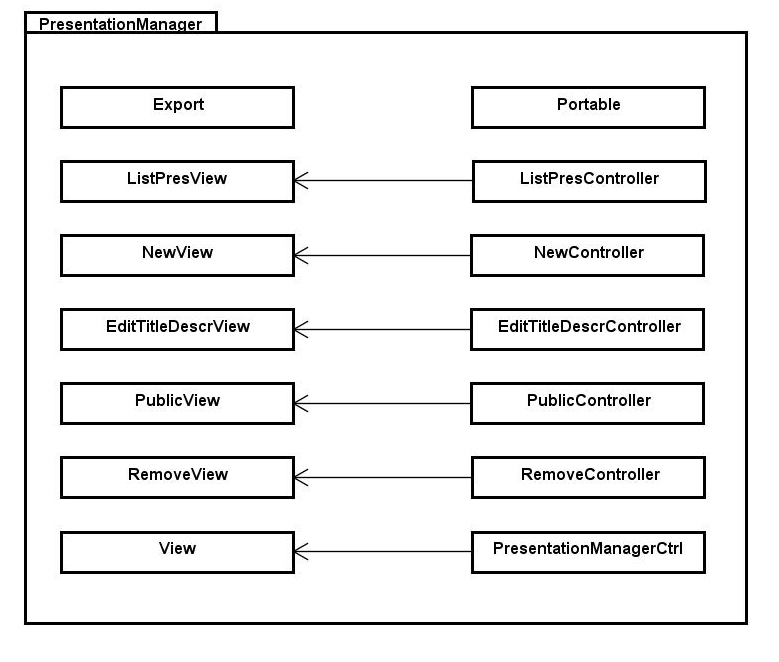
\includegraphics[scale=0.35]{img/diapkg/presentationmanager-class.jpg}
\caption{Diagramma del package Premi.PresentationManager}
\end{center}
\end{figure}
\begin{figure}[h!]
\begin{center}
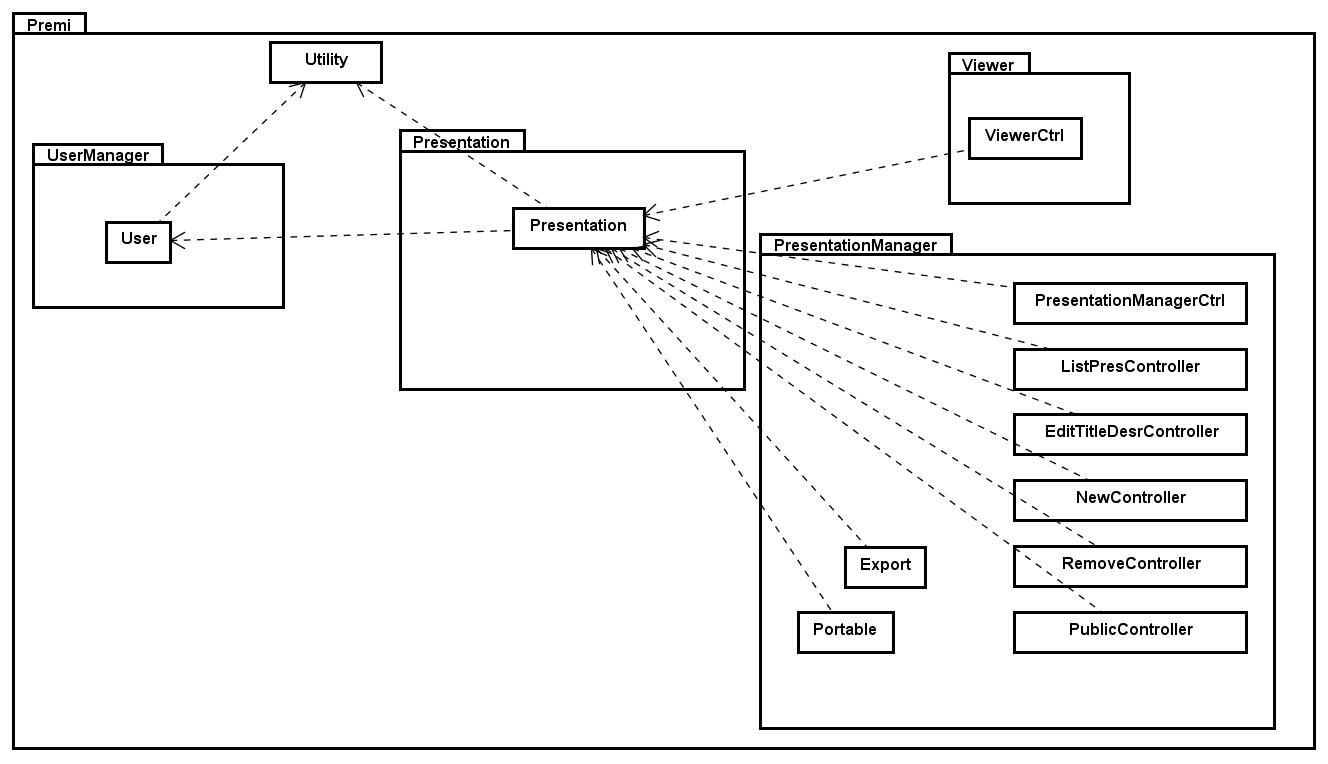
\includegraphics[scale=0.35]{img/diapkg/Completo_dettagliato.jpg}
\caption{Diagramma delle dipendenze delle classi di PresentationManager}
\end{center}
\end{figure}

\subsubsection{Premi.PresentationManager.Export}
\begin{itemize}
  \item \textbf{Nome:} Export 
  \item \textbf{Tipo:} class
  \item \textbf{Package:} Premi.PresentationManager
  \item \textbf{Descrizione:} permette di esportare la presentazione in formato poster
  \item \textbf{Relazioni con altri componenti:} preleva le informazioni da \code{Premi.Presentation.Presentation} per costruire il poster
\end{itemize}
\subsubsection{Premi.PresentationManager.Portable}
\begin{itemize}
  \item \textbf{Nome:} Portable
  \item \textbf{Tipo:} class
  \item \textbf{Package:} Premi.PresentationManager
  \item \textbf{Descrizione:} permette di rendere portabile una presentazione, e quindi di essere indipendente dal software Premi e di essere caricata come pagina HTML$_G$ da un browser$_G$
  \item \textbf{Relazioni con altri componenti:} preleva le informazioni da \code{Premi.Presentation.Presentation} per costruire la pagina HTML$_G$
\end{itemize}
\subsubsection{Premi.PresentationManager.View}
\begin{itemize}
  \item \textbf{Nome:} View
  \item \textbf{Tipo:} class
  \item \textbf{Package:} Premi.PresentationController
  \item \textbf{Descrizione:} è la view generale delle operazioni che l'utente puo' effettuare sulla sua lista di presentazioni
\end{itemize}
\subsubsection{Premi.PresentationManager.PresentationManagerCtrl}
\begin{itemize}
  \item \textbf{Nome:} PresentationManagerCtrl
  \item \textbf{Tipo:} class
  \item \textbf{Package:} Premi.PresentationManager
  \item \textbf{Descrizione:} fornisce alla view gli strumenti necessari alla gestione delle presentazioni
  \item \textbf{Relazioni con altri componenti:} è il controller dedicato di  \code{Premi.PresentationManager.View} 
\end{itemize}
\subsubsection{Premi.PresentationManager.RemoveView}
\begin{itemize}
  \item \textbf{Nome:} RemoveView
  \item \textbf{Tipo:} class
  \item \textbf{Package:} Premi.PresentationManager
  \item \textbf{Descrizione:} mostra una finestra di conferma eliminazione della presentazione selezionata
\end{itemize}
\subsubsection{Premi.PresentationManager.RemoveController}
\begin{itemize}
  \item \textbf{Nome:} RemoveController
  \item \textbf{Tipo:} class
  \item \textbf{Package:} Premi.PresentationManager
  \item \textbf{Descrizione:} fornisce alla view gli strumenti per rimuovere la presentazione o annullare l'azione
  \item \textbf{Relazioni con altri componenti:} è il controller dedicato di  \code{Premi.PresentationManager.RemoveView} e sfrutta le funzionalità di \code{Premi.Presentation.Presentation} per l'eliminazione della presentazione
\end{itemize}
\subsubsection{Premi.PresentationManager.PublicView}
\begin{itemize}
  \item \textbf{Nome:} PublicView
  \item \textbf{Tipo:} class
  \item \textbf{Package:} Premi.PresentationManager
  \item \textbf{Descrizione:} mostra una finestra di conferma per rendere pubblica o privata una presentazione
\end{itemize}
\subsubsection{Premi.PresentationManager.PublicController}
\begin{itemize}
  \item \textbf{Nome:} PublicController
  \item \textbf{Tipo:} class
  \item \textbf{Package:} Premi.PresentationManager
  \item \textbf{Descrizione:} fornisce alla view gli strumenti per rendere pubblica o privata una presentazione
  \item \textbf{Relazioni con altri componenti:} è il controller dedicato di  \code{Premi.PresentationManager.PublicView} e sfrutta le funzionalità di \code{Premi.Presentation.Presentation} per accedere alla base di dati
\end{itemize}
\subsubsection{Premi.PresentationManager.EditTitleDescrView}
\begin{itemize}
  \item \textbf{Nome:} EditTitleDescrView
  \item \textbf{Tipo:} class
  \item \textbf{Package:} Premi.PresentationManager
  \item \textbf{Descrizione:} mostra una finestra per la modifica del titolo e della descrizone della presentazione
\end{itemize}
\subsubsection{Premi.PresentationManager.EditTitleDescrController}
\begin{itemize}
  \item \textbf{Nome:} EditTitleDescrController
  \item \textbf{Tipo:} class
  \item \textbf{Package:} Premi.PresentationManager
  \item \textbf{Descrizione:} fornisce alla view la possibilità di modificare titolo e descrizione della presentazione
  \item \textbf{Relazioni con altri componenti:} è il controller dedicato di  \code{Premi.PresentationManager.EditTitleDescrView} e sfrutta le funzionalità di \code{Premi.Presentation.Presentation} per accedere alla base di dati
\end{itemize}
\subsubsection{Premi.PresentationManager.NewView}
\begin{itemize}
  \item \textbf{Nome:} NewView
  \item \textbf{Tipo:} class
  \item \textbf{Package:} Premi.PresentationManager
  \item \textbf{Descrizione:} mostra una finestra per la creazione di una nuova presentazione
\end{itemize}
\subsubsection{Premi.PresentationManager.NewController}
\begin{itemize}
  \item \textbf{Nome:} NewController
  \item \textbf{Tipo:} class
  \item \textbf{Package:} Premi.PresentationManager
  \item \textbf{Descrizione:} fornisce alla view gli strumenti per creare una nuova presentazione
  \item \textbf{Relazioni con altri componenti:} è il controller dedicato di  \code{Premi.PresentationManager.NewView} e sfrutta le funzionalità di \code{Premi.Presentation.Presentation} per accedere alla base di dati
\end{itemize}
\subsubsection{Premi.PresentationManager.ListPresView}
\begin{itemize}
  \item \textbf{Nome:} ListPresView
  \item \textbf{Tipo:} class
  \item \textbf{Package:} Premi.PresentationManager
  \item \textbf{Descrizione:} mostra all'utente la lista delle sue presentazioni, e bottoni aggiuntivi per accedere alle altre funzionalità del package$_G$
\end{itemize}
\subsubsection{Premi.PresentationManager.ListPresController}
\begin{itemize}
  \item \textbf{Nome:} ListPresController
  \item \textbf{Tipo:} class
  \item \textbf{Package:} Premi.PresentationManager
  \item \textbf{Descrizione:} fornisce alla view una lista preformata delle presentazioni dell'utente
  \item \textbf{Relazioni con altri componenti:} è il controller dedicato di  \code{Premi.PresentationManager.ListPresView} e sfrutta le funzionalità di \code{Premi.Presentation.Presentation} per recuperare la lista delle presentazioni
\end{itemize}



\clearpage
\subsection{Premi.Editor}
\begin{figure}[h!]
\begin{center}
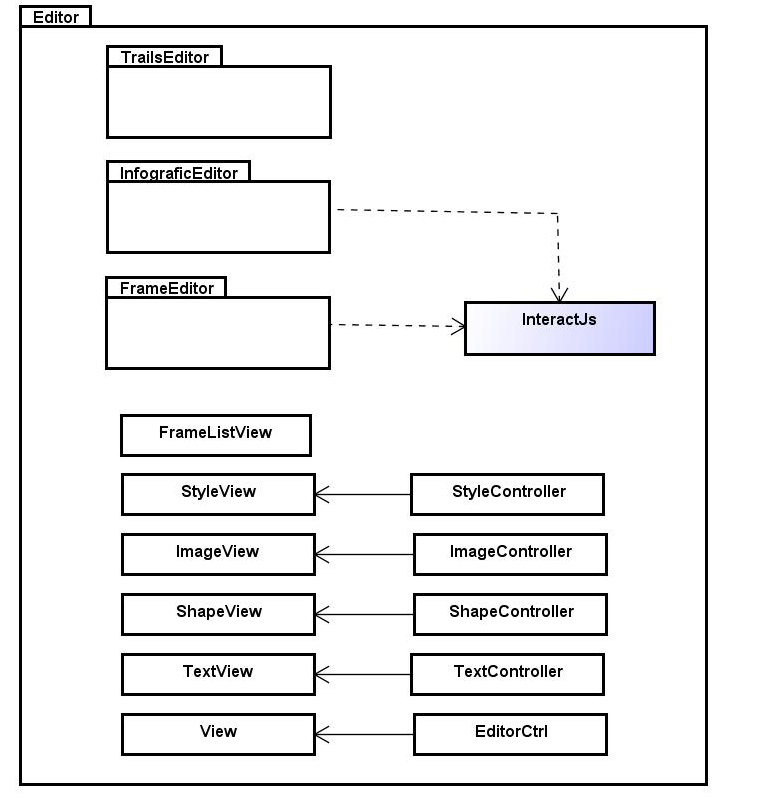
\includegraphics[scale=0.45]{img/diapkg/editor-class.jpg}
\caption{Diagramma del package Premi.Editor}
\end{center}
\end{figure}
\clearpage
\begin{figure}[h!]
\begin{center}
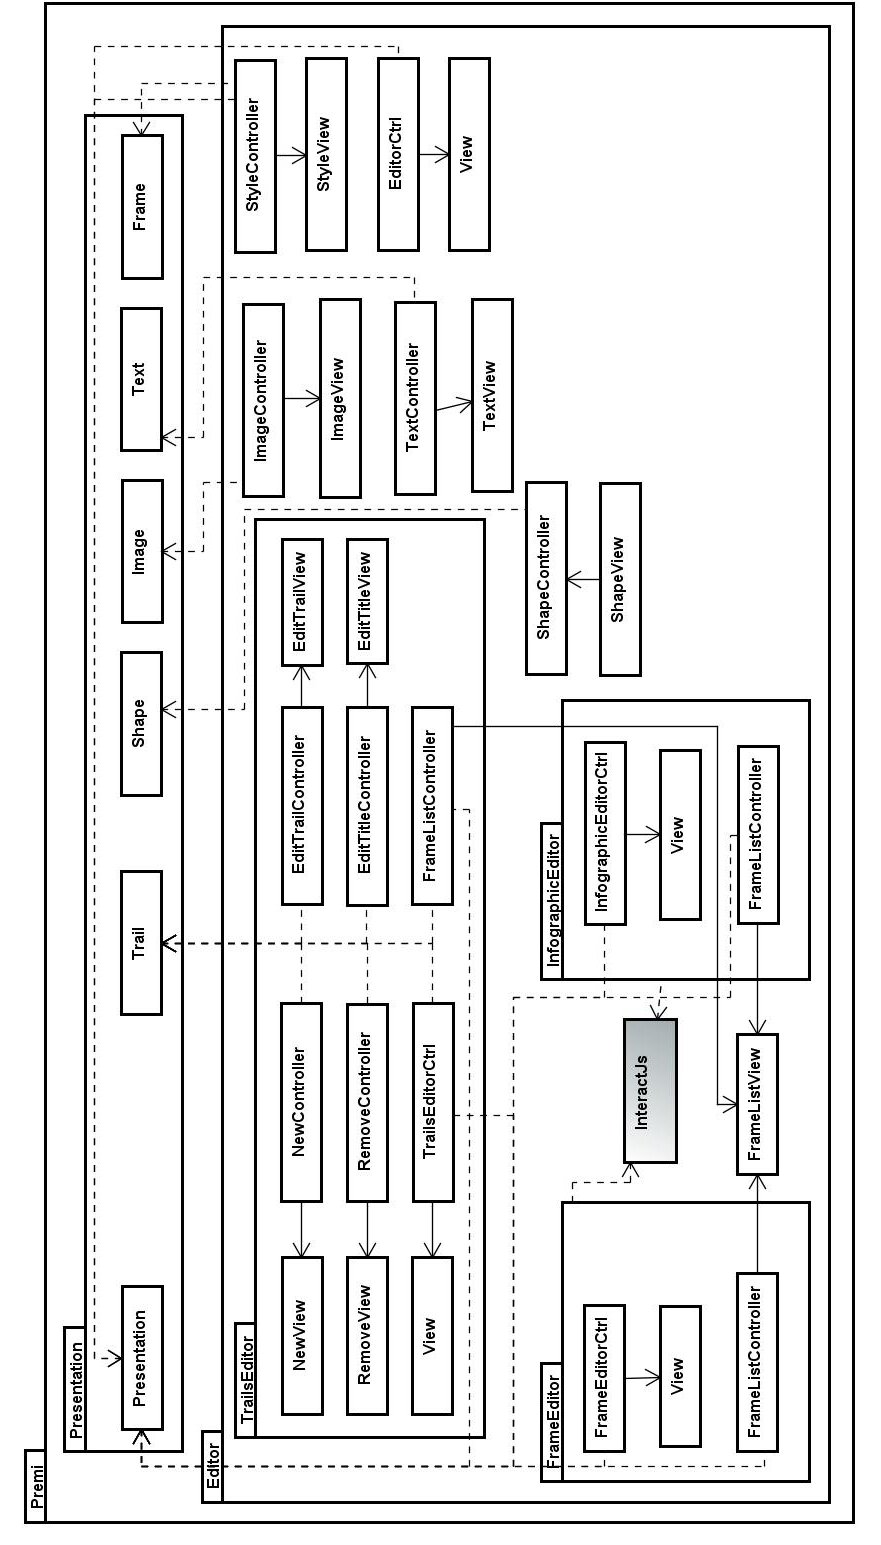
\includegraphics[scale=0.40]{img/diapkg/dettaglio_editor_presentation.jpg}
\caption{Diagramma delle classi di Premi.Editor e delle loro relazioni}
\end{center}
\end{figure}
\clearpage

\subsubsection{Premi.Editor.View}
\begin{itemize}
  \item \textbf{Nome:} View
  \item \textbf{Tipo:} class
  \item \textbf{Package:} Premi.Editor
  \item \textbf{Descrizione:} view generica dell'editor che funge da contenitore
\end{itemize}
\subsubsection{Premi.Editor.EditorCtrl}
\begin{itemize}
  \item \textbf{Nome:} EditorCtrl
  \item \textbf{Tipo:} class
  \item \textbf{Package:} Premi.Editor
  \item \textbf{Descrizione:} fornisce alla view le funzionzalità per la modifica di una presentazione
  \item \textbf{Relazioni con altri componenti:} è il controller dedicato di  \code{Premi.Editor.View} e sfrutta \code{Premi.Presentation.Presentation} per recuperare la presentazione dalla base di dati
\end{itemize}
\subsubsection{Premi.Editor.TextView}
\begin{itemize}
  \item \textbf{Nome:} TextView
  \item \textbf{Tipo:} class
  \item \textbf{Package:} Premi.Editor
  \item \textbf{Descrizione:} mostra le opzioni per l'aggiunta di un'area di testo
\end{itemize}
\subsubsection{Premi.Editor.TextController}
\begin{itemize}
  \item \textbf{Nome:} TextController
  \item \textbf{Tipo:} class
  \item \textbf{Package:} Premi.Editor
  \item \textbf{Descrizione:} fornisce alla view le funzionalità per creare e modificare un'area di testo
  \item \textbf{Relazioni con altri componenti:} è il controller dedicato di  \code{Premi.Editor.TextView} e utilizza la classe \code{Premi.Presentation.Text} per rappresentare le aree di testo
\end{itemize}
\subsubsection{Premi.Editor.ShapeView}
\begin{itemize}
  \item \textbf{Nome:} ShapeView
  \item \textbf{Tipo:} class
  \item \textbf{Package:} Premi.Editor
  \item \textbf{Descrizione:} mostra le opzioni per l'aggiunta di una figura
\end{itemize}
\subsubsection{Premi.Editor.ShapeController}
\begin{itemize}
  \item \textbf{Nome:} ShapeController
  \item \textbf{Tipo:} class
  \item \textbf{Package:} Premi.Editor
  \item \textbf{Descrizione:} fornisce alla view le funzionalità per creare e modificare una figura
  \item \textbf{Relazioni con altri componenti:} è il controller dedicato di  \code{Premi.Editor.ShapeView}  e utilizza la classe \code{Premi.Presentation.Shape} per rappresentare le figure
\end{itemize}
\subsubsection{Premi.Editor.ImageView}
\begin{itemize}
  \item \textbf{Nome:} ImageView
  \item \textbf{Tipo:} class
  \item \textbf{Package:} Premi.Editor
  \item \textbf{Descrizione:} mostra le opzioni per l'aggiunta di un'immagine
\end{itemize}
\subsubsection{Premi.Editor.ImageController}
\begin{itemize}
  \item \textbf{Nome:} ImageController
  \item \textbf{Tipo:} class
  \item \textbf{Package:} Premi.Editor
  \item \textbf{Descrizione:} fornisce alla view le funzionalità per aggiungere un'immagine
  \item \textbf{Relazioni con altri componenti:} è il controller dedicato di  \code{Premi.Editor.ImageView}  e utilizza la classe \code{Premi.Presentation.Image} per rappresentare le immagini
\end{itemize}
\subsubsection{Premi.Editor.StyleView}
\begin{itemize}
  \item \textbf{Nome:} StyleView
  \item \textbf{Tipo:} class
  \item \textbf{Package:} Premi.Editor
  \item \textbf{Descrizione:} permette la modifica dello stile di un Frame$_G$ oppure dello sfondo dell'infografica$_G$
\end{itemize}
\subsubsection{Premi.Editor.StyleController}
\begin{itemize}
  \item \textbf{Nome:} StyleController
  \item \textbf{Tipo:} class
  \item \textbf{Package:} Premi.Editor
  \item \textbf{Descrizione:} fornisce alla view le funzionalità per la modifica dello stile
  \item \textbf{Relazioni con altri componenti:} è il controller dedicato di  \code{Premi.Editor.StyleView},  e utilizza la classe \code{Premi.Presentation.Frame} per rappresentare lo stile dei Frame$_G$ e dell'infografica$_G$
\end{itemize}
\subsubsection{Premi.Editor.FrameListView}
\begin{itemize}
  \item \textbf{Nome:} FrameListView
  \item \textbf{Tipo:} class
  \item \textbf{Package:} Premi.Editor
  \item \textbf{Descrizione:} view di base per la rappresentazione di una lista dei Frame$_G$ contenuti all'interno della presentazione
\end{itemize}


\clearpage
\subsection{Premi.Editor.FrameEditor}
\begin{figure}[h!]
\begin{center}
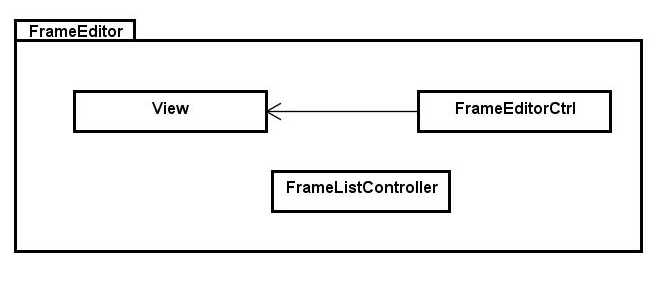
\includegraphics[scale=0.45]{img/diapkg/frameeditor-class.jpg}
\caption{Diagramma del package Premi.Editor.FrameEditor}
\end{center}
\end{figure}
\subsubsection{Premi.Editor.FrameEditor.View}
\begin{itemize}
  \item \textbf{Nome:} View
  \item \textbf{Tipo:} class
  \item \textbf{Package:} Premi.Editor.FrameEditor.View
  \item \textbf{Descrizione:} è la view generale della fase di modifica dei Frame$_G$
\end{itemize}
\subsubsection{Premi.Editor.FrameEditor.FrameEditorCtrl}
\begin{itemize}
  \item \textbf{Nome:} FrameEditorCtrl
  \item \textbf{Tipo:} class
  \item \textbf{Package:} Premi.Editor.FrameEditor.FrameEditorCtrl
  \item \textbf{Descrizione:} fornisce alla view le funzionalità per la gestione delle altre view contenute al suo interno
  \item \textbf{Relazioni con altri componenti:} è il controller dedicato di  \code{Premi.Editor.FrameEditor.View} ed elabora la presentazione tramite \code{Premi.Presentation.Presentation}
\end{itemize}
\subsubsection{Premi.Editor.FrameEditor.FrameListController}
\begin{itemize}
  \item \textbf{Nome:} FrameListController
  \item \textbf{Tipo:} class
  \item \textbf{Package:} Premi.Editor.FrameEditor
  \item \textbf{Descrizione:} fornisce alla view \code{FrameListView} le funzionalità per rappresentazione della lista dei Frame$_G$
  \item \textbf{Relazioni con altri componenti:} è uno dei tre controller dedicati di  \code{Premi.Editor.FrameListView}  e utilizza la classe \code{Premi.Presentation.Presentation} per prelevare i Frame$_G$ e crearne un'anteprima
\end{itemize}



\clearpage
\subsection{Premi.Editor.InfographicEditor}
\begin{figure}[h!]
\begin{center}
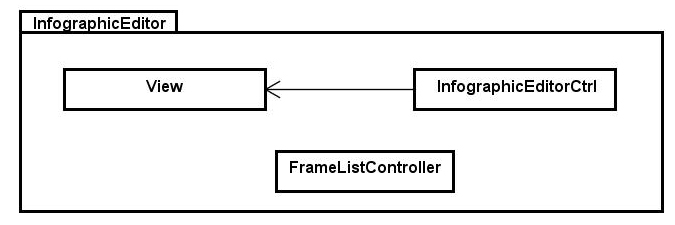
\includegraphics[scale=0.45]{img/diapkg/infographiceditor-class.jpg}
\caption{Diagramma del package Premi.Editor.InfographicEditor}
\end{center}
\end{figure}
\subsubsection{Premi.Editor.InfographicEditor.View}
\begin{itemize}
  \item \textbf{Nome:} View
  \item \textbf{Tipo:} class
  \item \textbf{Package:} Premi.Editor.InfographicEditor
  \item \textbf{Descrizione:}  è la view generale della fase di creazione o modifica dell'infografica$_G$
\end{itemize}
\subsubsection{Premi.Editor.InfographicEditor.InfographicEditorCtrl}
\begin{itemize}
  \item \textbf{Nome:} InfographicEditorCtrl
  \item \textbf{Tipo:} class
  \item \textbf{Package:} Premi.Editor.InfographicEditor
  \item \textbf{Descrizione:} fornisce alla view le funzionalità per la gestione delle altre view contenute al suo interno, che permetteranno all'utente di produrre un'infografica$_G$ attraverso l'utilizzo di oggetti grafici, tra cui i Frame$_G$ creati nella fase precedente
  \item \textbf{Relazioni con altri componenti:} è il controller dedicato di  \code{Premi.Editor.InfoGraphicEditor.View} ed elabora la presentazione tramite \code{Premi.Presentation.Presentation} 
\end{itemize}
\subsubsection{Premi.Editor.InfographicEditor.FrameListController}
\begin{itemize}
  \item \textbf{Nome:} FrameListController
  \item \textbf{Tipo:} class
  \item \textbf{Package:} Premi.Editor.InfographicEditor
  \item \textbf{Descrizione:} fornisce alla view \code{FrameListView} le funzionalità per rappresentazione della lista dei Frame$_G$
  \item \textbf{Relazioni con altri componenti:} è uno dei tre controller dedicati di  \code{Premi.Editor.FrameListView}  e utilizza la classe \code{Premi.Presentation.Presentation} per prelevare i Frame$_G$ e crearne un'anteprima
\end{itemize}



\clearpage
\subsection{Premi.Editor.TrailsEditor}
\begin{figure}[h!]
\begin{center}
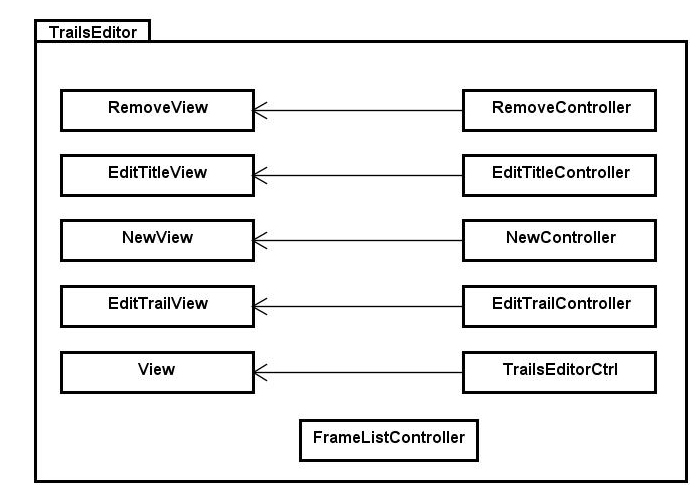
\includegraphics[scale=0.45]{img/diapkg/trailseditor-class.jpg}
\caption{Diagramma del package Premi.Editor.TrailsEditor}
\end{center}
\end{figure}
\subsubsection{Premi.Editor.TrailsEditor.View}
\begin{itemize}
  \item \textbf{Nome:} View
  \item \textbf{Tipo:} class
  \item \textbf{Package:} Premi.Editor.TrailsEditor
  \item \textbf{Descrizione:} view generale della della fase di creazione o modifica dei percorsi di presentazione
\end{itemize}
\subsubsection{Premi.Editor.TrailsEditor.TrailsEditorCtrl}
\begin{itemize}
  \item \textbf{Nome:} TrailsEditorCtrl
  \item \textbf{Tipo:} class
  \item \textbf{Package:} Premi.Editor.TrailsEditor
  \item \textbf{Descrizione:} fornisce alla view le funzionalità per la gestione delle altre view contenute al suo interno, che permetteranno di gestire i percorsi di presentazione
  \item \textbf{Relazioni con altri componenti:}  è il controller dedicato di  \code{Premi.Editor.TrailsEditor.View} , si collega a \code{Premi.Presentation.Presentation} per recuperare oggetti di tipo \code{Premi.Presentation.Trail}
\end{itemize}
\subsubsection{Premi.Editor.TrailsEditor.FrameListController}
\begin{itemize}
  \item \textbf{Nome:} FrameListController
  \item \textbf{Tipo:} class
  \item \textbf{Package:} Premi.Editor.TrailsEditor
  \item \textbf{Descrizione:} fornisce alla view \code{FrameListView} le funzionalità per rappresentazione della lista dei Frame$_G$
  \item \textbf{Relazioni con altri componenti:} è uno dei tre controller dedicati di  \code{Premi.Editor.FrameListView}  e utilizza la classe \code{Premi.Presentation.Presentation} per prelevare i Frame$_G$ e crearne un'anteprima
\end{itemize}
\subsubsection{Premi.Editor.TrailsEditor.EditTrailView}
\begin{itemize}
  \item \textbf{Nome:} EditTrailView
  \item \textbf{Tipo:} class
  \item \textbf{Package:} Premi.Editor.TrailsEditor
  \item \textbf{Descrizione:} view dedicata alla modifica di un percorso di presentazione
\end{itemize}
\subsubsection{Premi.Editor.TrailsEditor.EditTrailController}
\begin{itemize}
  \item \textbf{Nome:} EditTrailController
  \item \textbf{Tipo:} class
  \item \textbf{Package:} Premi.Editor.TrailsEditor
  \item \textbf{Descrizione:} fornisce alla view le funzionalità per la gestione delle altre view contenute al suo interno, che permetteranno all'utente di produrre un percorso di presentazione con i Frame da lui creati
  \item \textbf{Relazioni con altri componenti:} è il controller dedicato di  \code{Premi.Editor.TrailsEditor.EditTrailView} e modifica il percorso sfruttando la classe \code{Premi.Presentation.Trail}
\end{itemize}
\subsubsection{Premi.Editor.TrailsEditor.NewView}
\begin{itemize}
  \item \textbf{Nome:} NewView
  \item \textbf{Tipo:} class
  \item \textbf{Package:} Premi.Editor.TrailsEditor
  \item \textbf{Descrizione:} mostra la finestra di creazione di un percorso di presentazione
\end{itemize}
\subsubsection{Premi.Editor.TrailsEditor.NewController}
\begin{itemize}
  \item \textbf{Nome:} NewController
  \item \textbf{Tipo:} class
  \item \textbf{Package:} Premi.Editor.TrailsEditor
  \item \textbf{Descrizione:} fornisce alla view le funzionalità per la creazione di un nuovo percorso di presentazione
  \item \textbf{Relazioni con altri componenti:} è il controller dedicato di  \code{Premi.Editor.TrailsEditor.NewView} e crea il nuovo percorso sfruttando la classe \code{Premi.Presentation.Trail}
\end{itemize}
\subsubsection{Premi.Editor.TrailsEditor.EditTitleView}
\begin{itemize}
  \item \textbf{Nome:} EditTitleView
  \item \textbf{Tipo:} class
  \item \textbf{Package:} Premi.Editor.TrailsEditor
  \item \textbf{Descrizione:} mostra la finestra di modifica del titolo di un percorso di presentazione
\end{itemize}
\subsubsection{Premi.Editor.TrailsEditor.EditTitleController}
\begin{itemize}
  \item \textbf{Nome:} EditTileController
  \item \textbf{Tipo:} class
  \item \textbf{Package:} Premi.Editor.TrailsEditor
  \item \textbf{Descrizione:} fornisce alla view le funzionalità per la modifica del titolo di un percorso di presentazione
  \item \textbf{Relazioni con altri componenti:} è il controller dedicato di  \code{Premi.Editor.TrailsEditor.EditTitleView} e modifica il titolo del percorso sfruttando la classe \code{Premi.Presentation.Trail}
\end{itemize}
\subsubsection{Premi.Editor.TrailsEditor.RemoveView}
\begin{itemize}
  \item \textbf{Nome:} RemoveView
  \item \textbf{Tipo:} class
  \item \textbf{Package:} Premi.Editor.TrailsEditor
  \item \textbf{Descrizione:} mostra la finestra di conferma rimozione di un percorso di presentazione
\end{itemize}
\subsubsection{Premi.Editor.TrailsEditor.RemoveController}
\begin{itemize}
  \item \textbf{Nome:} RemoveController
  \item \textbf{Tipo:} class
  \item \textbf{Package:} Premi.Editor.TrailsEditor
  \item \textbf{Descrizione:} fornisce alla view le funzionalità per la rimozione di un percorso di presentazione
  \item \textbf{Relazioni con altri componenti:} è il controller dedicato di  \code{Premi.Editor.TrailsEditor.RemoveView} 
\end{itemize} e rimuove il percorso sfruttando la classe \code{Premi.Presentation.Trail}












